\documentclass[../main]{subfiles}

\graphicspath{{../figures/}}

\begin{document}

\section{屋外実験}
\label{sec:outdoor_experiment}
本研究では,実験室内での評価に加え,より実環境に近い条件下で提案手法の性能を検証するため,石油精製プラント内での屋外実験を実施した.
以下では,実験環境の概要,実験手法,データの処理方法,得られた結果,そしてそれらに基づく考察について順に述べる.
\subsection{実験環境}
\label{subsec:vexp_ci_environment}
実験は,\reffig{fig:field_environment}に示す石油精製プラントの一角で実施した.
このエリアには,連続的に作動するポンプ類や定期的に圧力を放出するバルブ類など,複数の騒音源が点在している.
定期的に圧力を放出するバルブ類が点在している.作業日当日もプラント全体が通常稼働中であり,背景騒音は実験室よりも格段に大きい環境であった.

\begin{figure}[t]
  \centering
  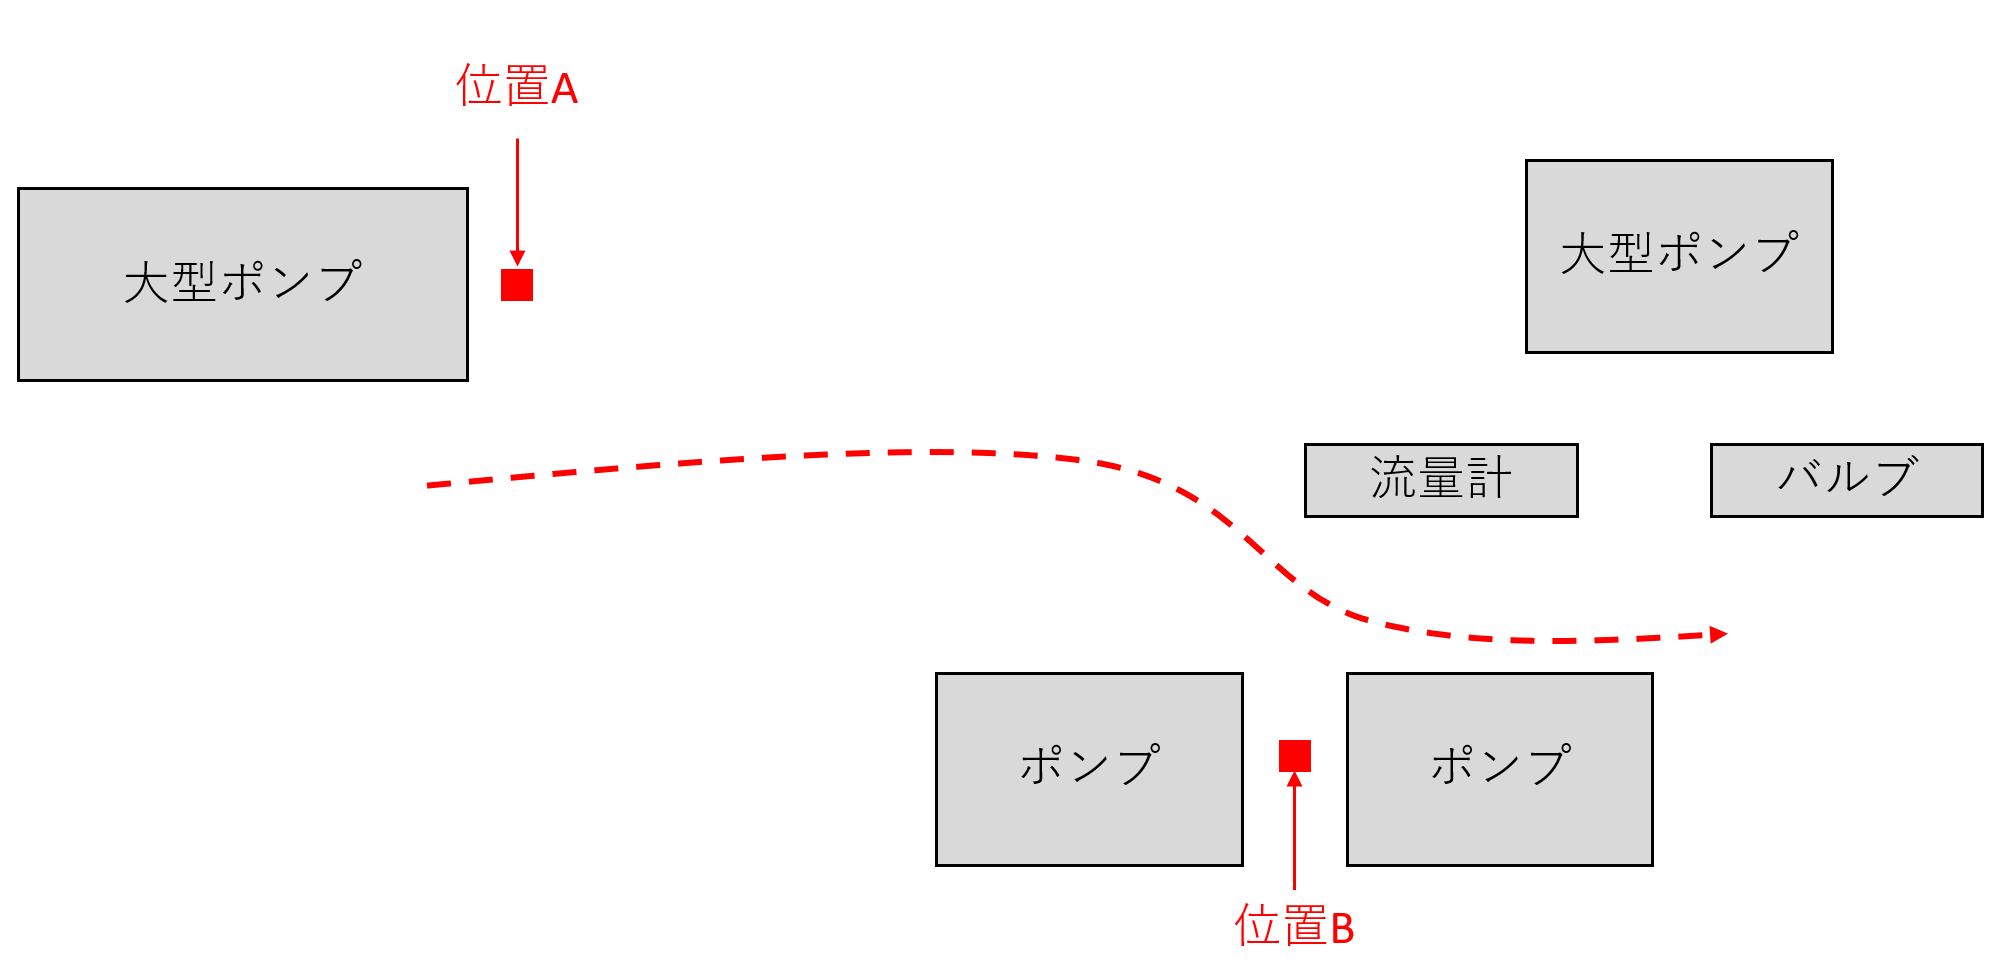
\includegraphics[keepaspectratio, width=1.0\linewidth]{chap4/field_environment.png}
  \caption{屋外実験における実験環境}
  \label{fig:field_environment}
\end{figure}

\subsection{実験方法}
\label{subsec:vexp_ci_method}
実験は,\reffig{fig:field_experimental_setup}に示すように,ポンプのような音源が存在する区間に経路を設定し,
\begin{figure}[t]
  \centering
  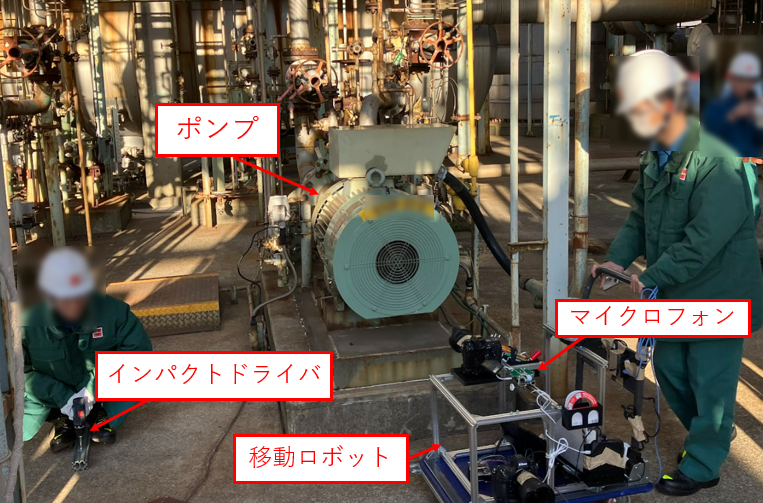
\includegraphics[keepaspectratio, width=0.7\linewidth]{chap4/field_experimental_setup.png}
  \caption{屋外実験の様子}
  \label{fig:field_experimental_setup}
\end{figure}



プラント内を走行する移動ロボットに音声収録用のマイクと信号処理装置を搭載し,走行経路上の音データを取得した.
まず,異常音源を配置しない状態で複数回走行し,プラントが正常稼働中の音を「正常サンプル」として収集した.
次に,異常音を模擬するため,インパクトドライバと金属棒の打撃装置をプラント内の2箇所に設置し,位置を切り替えながら追加の走行を行った.

\subsubsection{移動ロボットの自己位置推定}
移動ロボットの車輪にエンコーダを取り付け,それらのエンコーダから得られる回転角度の情報を用いてオドメトリを計算した.
具体的には,ロボットの左右の車輪の回転角度差から回転角と回転半径を求めることができ,これらの情報から微小時刻$\Delta t$におけるロボットの位置と姿勢の変化を算出することができる.
これを$\Delta t$ごとに積算することで,ロボットの現在位置を推定した.

\subsubsection{異常音の再現手法}
異常音としては,インパクトドライバによる連続的な衝撃音と,金属棒を打ち鳴らす周期的な打撃音を用いた.
これら2種類の音源を\reffig{fig:field_environment}に示す地点Aと地点Bに配置し,それぞれの配置を切り替えながら走行実験を実施した.
こうすることで,連続的な衝撃音(インパクトドライバ)と間欠的な打撃音(金属棒)という異なる種類の異常を再現した.
また,打撃音は1分間に240回のペースで2本の金属棒を打ち付けあうことで,異常音を再現した.
正常時の走行を3回,異常音源が存在する状態の走行を2回実施した.\reftab{tab:abnormal_sound_jp}にそれぞれの走行における異常音源を示す.
このとき,プラントが通常稼働状態であるため,背景騒音にはポンプやバルブなど多種多様な音が混在している.


\begin{table}[htbp]
  \centering
  \caption{各走行の異常音源の配置}
  \label{tab:abnormal_sound_jp}
  \begin{tabular}{c|c|c}
  \hline
   & \textbf{地点A} & \textbf{地点B} \\ \hline
  \textbf{1回目} & 金属棒を打撃 & インパクトドライバ \\
  \textbf{2回目} & インパクトドライバ & 金属棒を打撃 \\ \hline
  \end{tabular}
\end{table}

\subsection{データの処理}
\label{subsec:vexp_ci_processing}
取得した音声信号は,実験室での評価時と同様に48kHzのサンプリングレートで録音した.
まず,ノイズ除去や正規化などの基本的な前処理を行い,続いて短時間フーリエ変換によってスペクトログラムを得た.
メルフィルタバンクを用いることで周波数帯域を圧縮し,特徴量次元を削減した.
正常走行で収集したサンプルのうち一部を学習用データとし,残りの正常サンプルと異常サンプルを用いて提案手法をテストした.

\subsection{実験結果}
\label{subsec:vexp_ci_result}
屋外環境での実験結果を\reffig{fig:field_normal},\reffig{fig:field_abnormal1},および\reffig{fig:field_abnormal}に示す.
異常音源を設置していない走行時は,ほとんどのサンプルが正常音として正しく分類された.
一方,インパクトドライバや金属棒打撃装置が作動している走行時は,音源付近で異常として判定されるサンプルが明確に増加した.
インパクトドライバのように連続的な衝撃音を発する機器では,周辺エリアのサンプルが一貫して高い異常判定率を示した.
金属棒打撃のような間欠的な音源の場合は,打撃が行われるタイミングで局所的に異常判定が発生する傾向が観察された.
\begin{figure}[t]
  \centering
  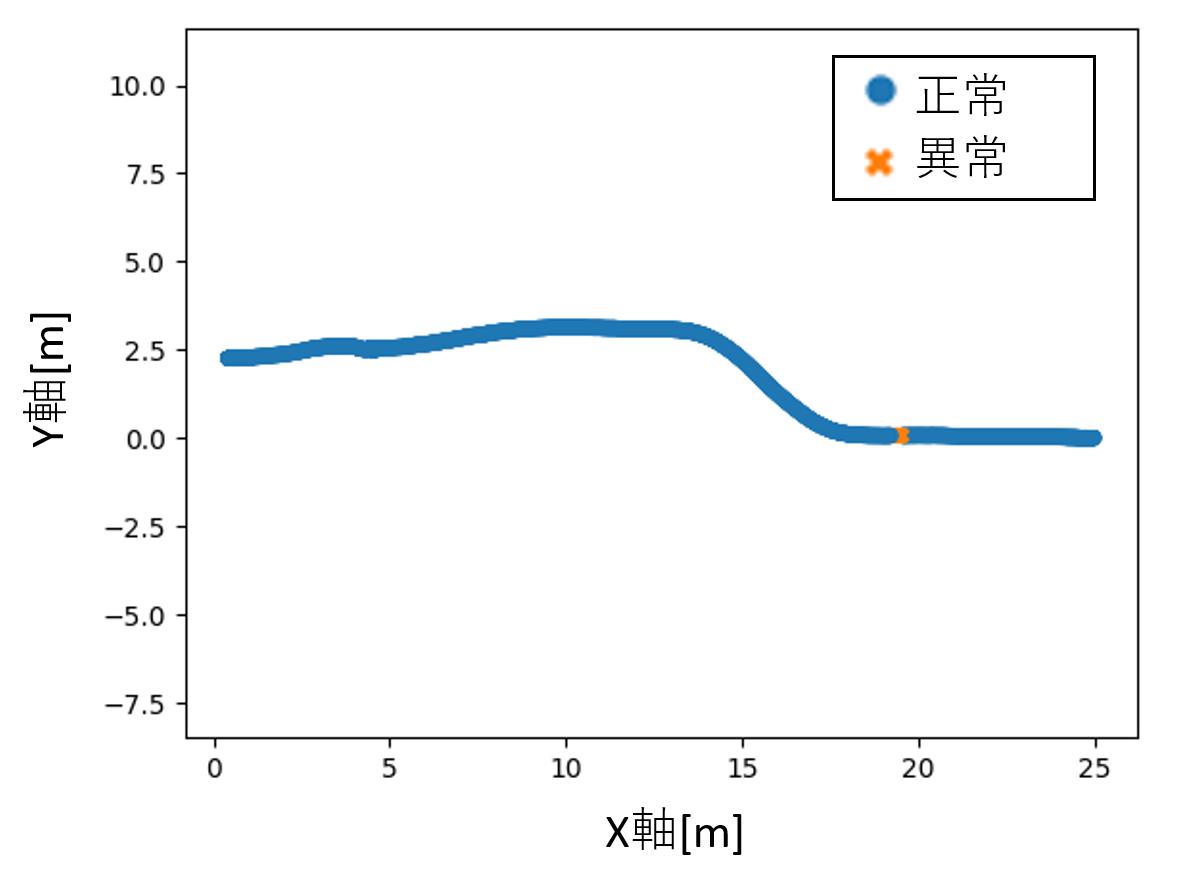
\includegraphics[keepaspectratio, width=0.7\linewidth]{chap4/field_normal.png}
  \caption{正常状態における異常検知結果}
  \label{fig:field_normal}
\end{figure}


\begin{figure}[t]
  \centering
  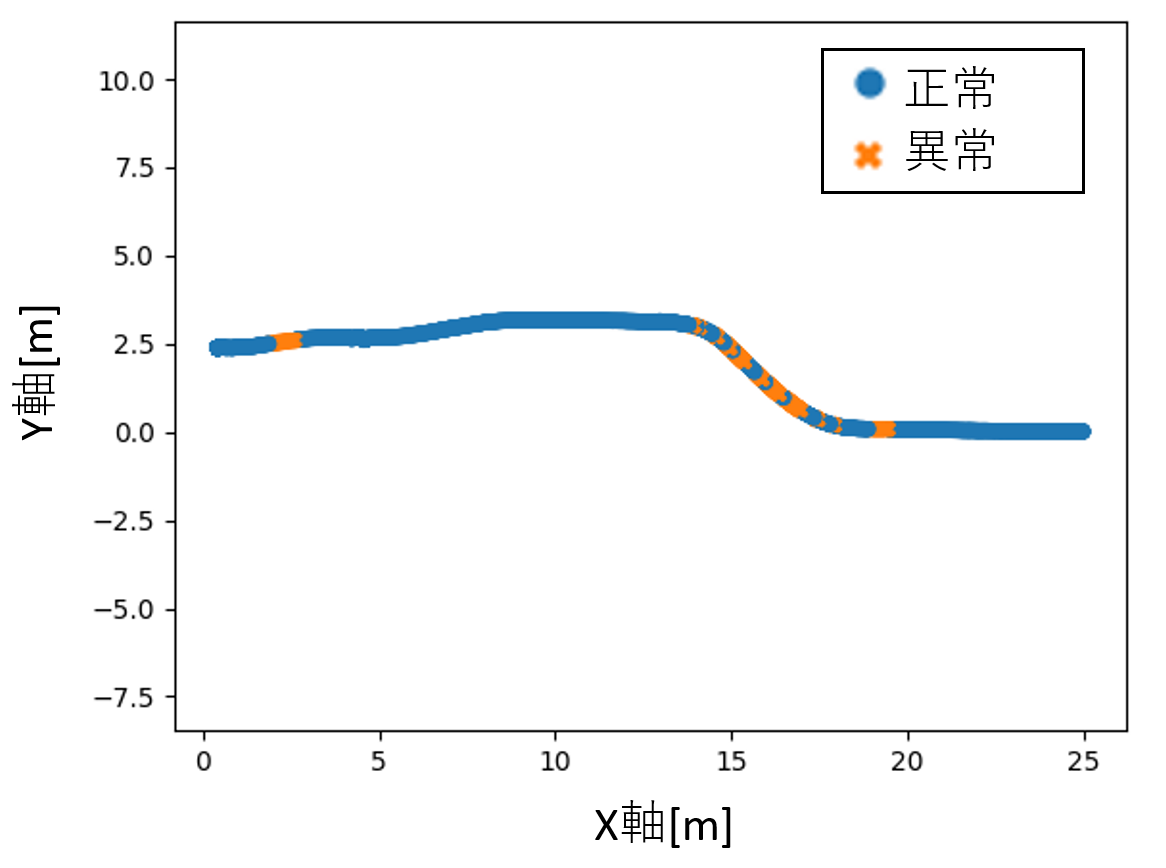
\includegraphics[keepaspectratio, width=0.7\linewidth]{chap4/field_abnormal1.png}
  \caption{異常状態における異常検知結果}
  \label{fig:field_abnormal1}
\end{figure}

\begin{figure}[t]
  \centering
  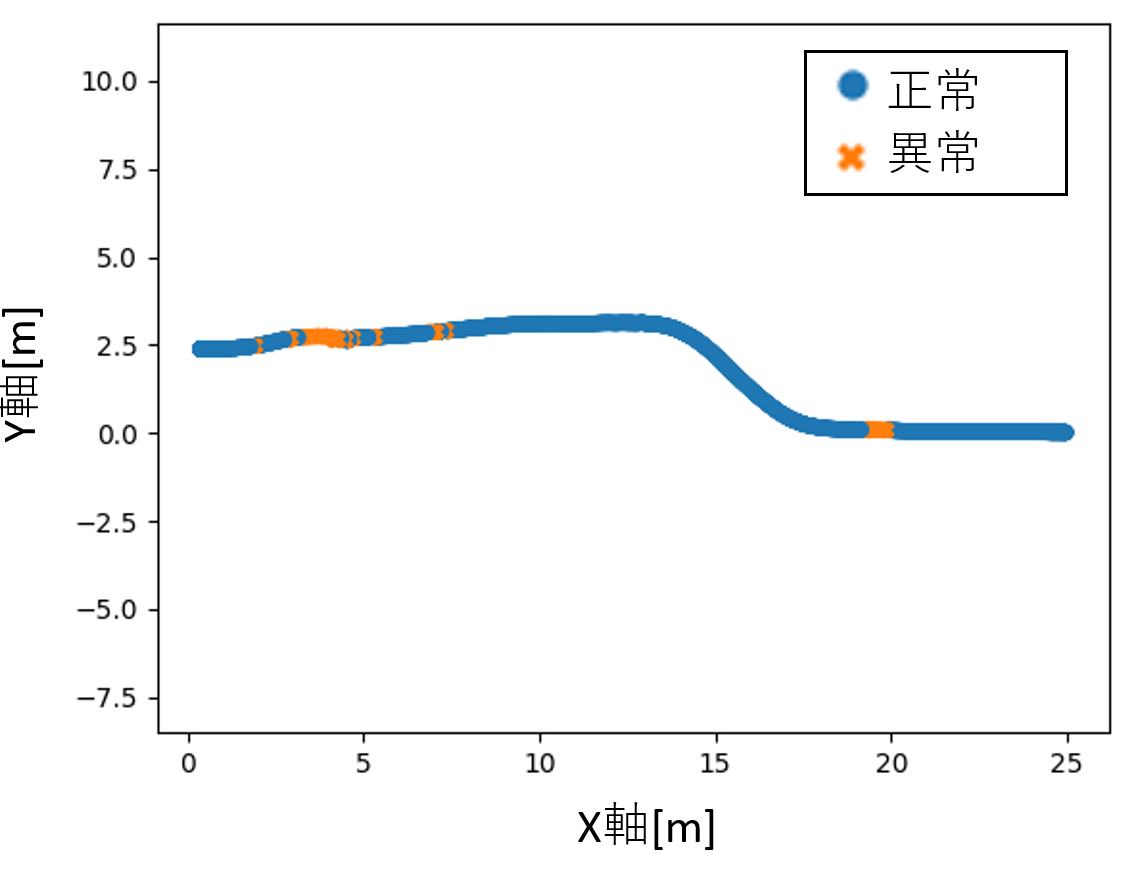
\includegraphics[keepaspectratio, width=0.7\linewidth]{chap4/field_abnormal.png}
  \caption{異常状態における異常検知結果}
  \label{fig:field_abnormal}
\end{figure}


\subsection{考察}

屋外実験の結果,プラント内の大きな背景騒音下においても,提案手法が異常音を検出できることが示唆された.
\reffig{fig:field_normal}からわかるように,異常音源を設置していない走行時は,ほとんどのフレームにおいて,正常音として正しく分類された.
このことから,提案手法が背景騒音が非常に大きい環境においても正常音のマッピングを適切に行っていることがわかる.
しかし,\reffig{fig:field_normal}では,正常な音を異常として判定する偽陽性が確認できる.
この原因として移動ロボットの走行音が挙げられる.
屋内実験では移動ロボットに凹凸の少ない地面を走行させたが,屋外実験ではアスファルトのような凹凸の大きい環境での走行となった.
このため,ロボットの走行音が大きくなり,学習データ,テストデータ共に正常音が不安定となってしまったことが原因として考えられる.
移動ロボットの走行音を除去することで,正常音の予測の精度向上と,偽陽性を減らしていくことが今後の課題の一つである.

一方で,\reffig{fig:field_abnormal1}および\reffig{fig:field_abnormal}を確認すると,間欠的な金属棒の打撃音の付近では,局所的に異常が観測されていることが分かる.
この結果から,金属棒の打撃と対応しているフレームのみが異常として判定されていることが考えられる.
これは異常音のエネルギーを決定する要因に距離以外のフレームと間欠的な音という別の要因が加わってしまうことを示唆しており,異常音が間欠的な特徴を持つ場合異常の位置推定が失敗することが考えられる.
このため,間欠的な異常音に対しても,異常の位置推定を可能とするような手法の開発が今後の課題となる.

\end{document}
